This section addresses the work progress within the ME. Refer to Sean Keene's thesis to get how the system is set up. This document, however, addresses an issue that is related to GridAPPS-D flexibility. 

\subsection{Problem Statement}

\begin{figure}[htp!]
    \centering
    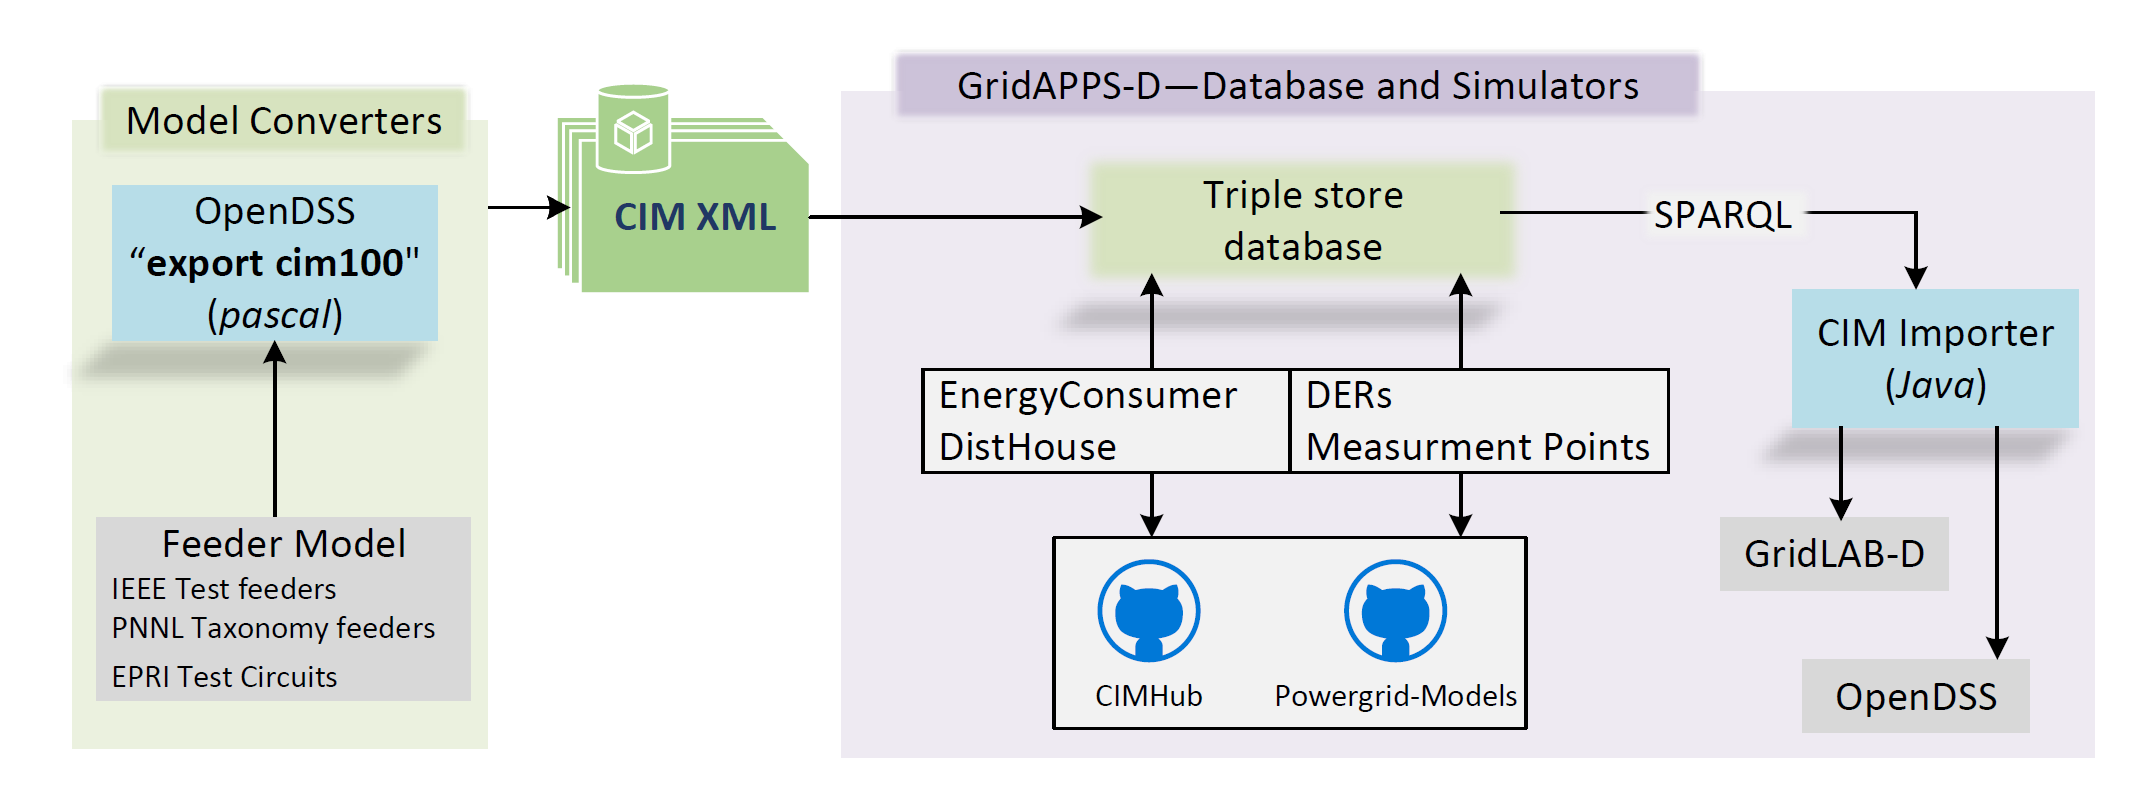
\includegraphics[width=0.7\columnwidth]{Pictures/model_conversion.png}
    \caption{GridAPPS-D Model Conversion}
    \label{fig:me_gridappsd}
\end{figure}

As shown in Figure~\ref{fig:me_gridappsd}, GridAPPS-D takes an input file (IEEE Test Feeders, PNNL Taxonomy Feeders, or EPRI Test Circuits) as a \textbf{dss} format. Within each \textbf{dss} file,
''export cim100'' command is used to export an XML version of the \textbf{dss} file. The XML file is then stored in the Triple Store database so it can be adjusted as needed. 


Over the years, the PowerLab team has been extensively working with GridLAB-D. The PowerLab team has developed several \textbf{glm} scripts to implement studies and cases. Many of these studies are slightly or non-GridAPPS-D-related. 
The time has come to merge many of these studies within the Modelling Environment (ME). This Section is meant to walk through the progress of implementing scripts that convert \textbf{glm} files to \textbf{dss}.

\subsection{Objectives}
\begin{itemize}
    \item Convert \textbf{glm} files to \textbf{Common Information Model (CIM)}.
    \item Insert the appropriate loads in the specified \textbf{glm} file using GridAPPS-D.
    \item Develop communication between entities and demand response capabilities.
\end{itemize}

\subsection{Tools to be Used}

\begin{itemize}
    \item To convert from GridLAB-D to OpenDSS, I used \href{https://github.com/NREL/ditto}{Ditto-CLI}
    \item To edit the \textbf{glm} files, I used \href{https://github.com/NREL/glm}{glm} module in Python.
    \item To convert from \textbf{dss} to \textbf{CIM}, I used \href{https://cimhub.readthedocs.io/en/latest/Tutorial.html#ieee-123-bus-base-case}{CIMhub}
\end{itemize}

\subsection{Processing Steps}

\begin{figure}[htp!]
    \centering
    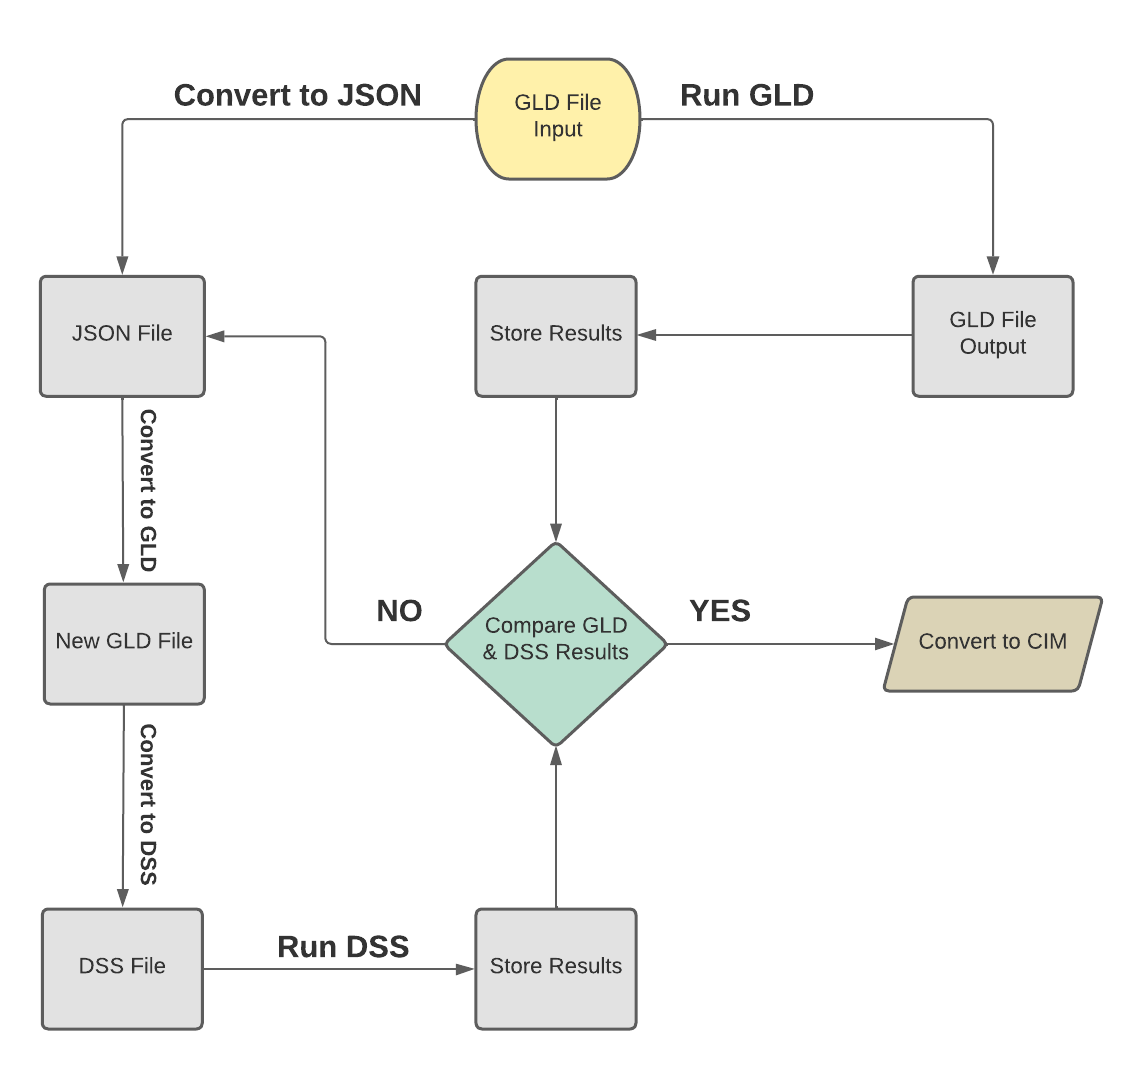
\includegraphics[width=0.7\columnwidth]{Pictures/glm_conversion_tool.png}
    \caption{File Conversion Processing Chart}
    \label{fig:me_conversion}
\end{figure}

\subsubsection{Step 1: Edit \textbf{glm} Files}

GridLAB-D and OpenDSS are different software packages and, therefore, they are not expected to have the same models. To find out which GridLAB-D objects are compatible with OpenDSS models, I went through test files 
within \href{https://github.com/NREL/ditto}{Ditto-CLI}. The \href{run:/home/deras/Desktop/Midrar_work/ditto/tests/data/small_cases/gridlabd/ieee_4node/node.glm}{Node.glm} is a \textbf{glm} file that can be easily 
converted to \textbf{dss} without errors. The content of this file is compared with the \textbf{glm} that I developed to ensure a smooth and accurate transition between GridLAB-D and OpenDSS. These models are as follows:

\begin{itemize}
    \item Clock
    \item module powerflow
    \item overhead line conductor
    \item line spacing
    \item line configuration
    \item transformer configuration
    \item node object
    \item overhead line object
    \item transformer objects
    \item load object
\end{itemize}

Note that objects like triplex load and water heaters are not included. Whether these objects can be implemented or not is not the question. The question is, 
do they align with the final objective of this work? Given that \textbf{CIM} files are general models, and their behavior mimics the operation of the aforementioned loads,
then the answer is no, they are not needed. 

To delete such objects from the GridLAB-D file (or \textbf(glm) file), we need a tool to access the \textbf(glm) file and perform the required edits. This editor as far as 
the author's knowledge does not exist. Therefore, I used the \href{https://github.com/NREL/glm}{GLM} module in Python. module in python. This module converts \textbf(glm) files to JSON and vice-versa. It's easy to deal with 
JSON files with python. Once the \textbf(glm) file is converted to JSON, the following objects were deleted:
\begin{itemize}
    \item triplex\_load objects.
    \item triplex\_line objects.
    \item house objects.
    \item waterheater objects.
    \item multi\_recoreder objects.
    \item player objects.
    \item capacitor objects.
\end{itemize}

Again, as far as the author's knowledge, these objects do not have similar models in OpenDSS. The next step is to convert the JSON file back to a \textbf(glm) format. There are 
several crucial factors to note here:

\begin{itemize}
    \item During the conversion process, the \textit(clock) object has double quotes instead of single quotes. GridLAB-D compiler does not interpret the double quotes correctly, so they need to 
    be changed to single quotes.
    \item The 13-node feeder contains 13 nodes. However, only 10 nodes are used due to reasons mentioned in \href{https://pdxscholar.library.pdx.edu/open_access_etds/6101/}{Midrar's Thesis}.
    Some branch nodes are not used within the 13-node feeder and these are as follows:
    \begin{itemize}
        \item Node 6711
        \item Node 6321
        \item Node 634
        \item Node 650
        \item Node 630
    \end{itemize}
\end{itemize}
To ensure an accurate and smooth conversion from GridLAB-D to OpenDSS, run the \textbf(glm) file and the \textbf(dss) file and make sure they run correctly without errors and have the same
results.

\subsubsection{Ditto-CLI}
To convert a \textbf{glm} file to \textbf{dss}, the following command may be used:
\begin{lstlisting}[language=bash]
    $ ditto-cli convert --input ``glm file name'' --from gridlabd --to opendss --output ``output file directory''
\end{lstlisting}

The \href{https://github.com/NREL/ditto}{Ditto-CLI} tool does most of the work for those who want to convert GridLAB-D files to OpenDSS and vice-versa. However, it is not perfect and it has its 
shortfalls. several errors in particular that have been showing most of the time are the following:
\begin{lstlisting}[language=python]
    $ Matrix Inversion Error for Line ``line name''.
    $ TLineObj.CalcYPrim.
    $ Access violation.
\end{lstlisting}
Such errors are caused by the length and impedance conversions of the overhead and underground lines. In my case, since I'm working on the 13-node feeder, I need to make sure the original length
parameters and impedance matrices are the same as the one I have. After the conversion, run the \textbf{dss} file and if it outputs similar errors as above, do the following:
\begin{itemize}
    \item edit ``LineCodes.dss'' file.
    \item change the ``R'' and ``X'' matrices and ensure they correspond to the original IEEE-13 Node Feeder.
    \item All original IEEE feeders in \textbf{dss} format can be found in \href{https://github.com/tshort/OpenDSS/tree/master/Distrib/IEEETestCases}{DSS Github Repository}
\end{itemize}

\subsection{Important opendsscmd Commands}
\begin{itemize}
    \item To export an XML version of the current \textbf{dss} feeder, insert the following command within the ``Master.dss'' file:
    \begin{lstlisting}[language=python]
        $ export cim100
    \end{lstlisting}
    \item To export a CIM version of the current \textbf{dss} file, create a script containing the following and name it ``export\_cim.dss'':
    \begin{lstlisting}[language=python]
        redirect Master.dss
        solve
        export y triplet base_ysparse.csv
        export ynodelist base_nodelist.csv
        export summary base_summary.csv
    \end{lstlisting}
    \item Using opendsscmd command in the terminal, run the above script.
    \item \href{https://sourceforge.net/projects/electricdss/files/OpenDSSCmd/}{Source of the above info}.
\end{itemize}
